\documentclass[polish,polish,a4paper]{article}
\usepackage[T1]{fontenc}
\usepackage{polski}
\usepackage[utf8]{inputenc}
\usepackage{babel}
\usepackage{pslatex}
\usepackage{graphicx}
\usepackage{tikz}
\usepackage{pgfplots}
\usepackage{anysize}
\usepackage{pgfgantt}
\usepackage{latexsym,amsmath}
\usepackage{hyperref}
\marginsize{2.5cm}{2.5cm}{3cm}{3cm}



\newcommand{\name}[1]{\sffamily\bfseries\scriptsize #1}

\newcommand{\frontpage}[8]{
%% #1 - nazwa kursu
%% #2 - kierunek 
%% #3 - termin 
%% #4 - temat 
%% #5 - problem
%% #6 - skład grupy
%% #7 - nr grupy
%% #8 - data

\hfill
\includegraphics[width=4cm]{PWr.png}
\vspace{2cm}

\begin{tabular}{|p{0.72\textwidth}|p{0.28\textwidth}|}
\hline
\multicolumn{2}{|c|}{}\\
\multicolumn{2}{|c|}{{\LARGE #1}}\\
\multicolumn{2}{|c|}{}\\
\hline
\name{Kierunek} & \name{Termin}\\
\multicolumn{1}{|c|}{\textit{#2}} & \multicolumn{1}{|c|}{\textit{#3}} \\
\hline
\name{Temat} & \name{data}\\
\multicolumn{1}{|c|}{\textit{#4}} & \multicolumn{1}{|c|}{\textit{#5}} \\
\hline
\name{Grupa oddająca projekt} & \name{Nr indeksu}\\
\multicolumn{1}{|c|}{\textit{#6}} & \multicolumn{1}{|c|}{\textit{#7}} \\
\hline
\end{tabular}
}

\usepackage{listings}
\usepackage{xcolor} % for setting colors

% set the default code style
\lstset{
    frame=tb, % draw a frame at the top and bottom of the code block
    tabsize=4, % tab space width
    showstringspaces=false, % don't mark spaces in strings
    numbers=left, % display line numbers on the left
    commentstyle=\color{green}, % comment color
    keywordstyle=\color{blue}, % keyword color
    stringstyle=\color{red} % string color
}




\title{Sprawozdanie SPD}
\pgfplotsset{compat=1.16}
\begin{document}
% #1 - nazwa kursu #2 - kierunek  #3 - termin #4 - temat #5 - data #6 - skład grupy #7 - nr grupy
\frontpage{Bazy danych 2}{Informatyka}{Czwartek 17:05}{Projekt biura podróży}{\today}{Paweł Sagan, Patryk Wlazłyń}{241250, 241249}
\pagestyle{}
\newpage
\section{Wstęp}
Celem projektu było zaprojektowanie oraz stworzenie systemu bazodanowego. Stworzona przez nas aplikacja jest systemem biura podróży, umożliwiającym zarządzanie wycieczkami, klientami oraz pracownikami wspomnianej firmy. Wyróżniamy podział na dwie kategorie gracowników, manager oraz zwykły pracownik biura. Posiadają oni różne uprawnienia do wykonywanych operacji w systemie. Aplikacja obsługuje różnego rodzaju powiadomienia wysyłane do klientów, dzięki czemu możliwe jest informowanie ich o zbliżających się wycieczkach.Program umożliwia tworzenie statystyk przychodów firmy. System zakłada, iż rejestrowanie wycieczek, klientów oraz transakcji odbywa się za pośrednictwem pracownika biura podróży.
\section{Specyfikacja wymagań i diagram związków encji}
\subsection{Wymagania funkcjonalne i niefunkcjonalne}

Funkcjonalne:
\begin{itemize}
  \item Dodawanie, usuwanie, modyfikacje nowych klientów, ofert wycieczek i pracowników.
  \item Wykupywanie wycieczek przez klientów (przypisanie klienta to wycieczki, rejestrowanie wpłaconych pieniędzy)
  \item Wyszukiwanie wycieczek według kryteriów podanych przez klienta tj. kraj, cena...
  \item Powiadomienie na Emil o zbliżającym się terminie zapłaty i wycieczki
\end{itemize}
Niefunkcjonalne:
\begin{itemize}
  \item Interfejs dla pracownika biura podroży do obsługi klientów zainstalowany na komputerze pracownika (GUI QT).
  \item Użycie C++ do komunikacji z baza danych (mysql, mariadb) oraz do tworzenia interfejsu.
\end{itemize}
\subsection{Diagram przypadków użycia}
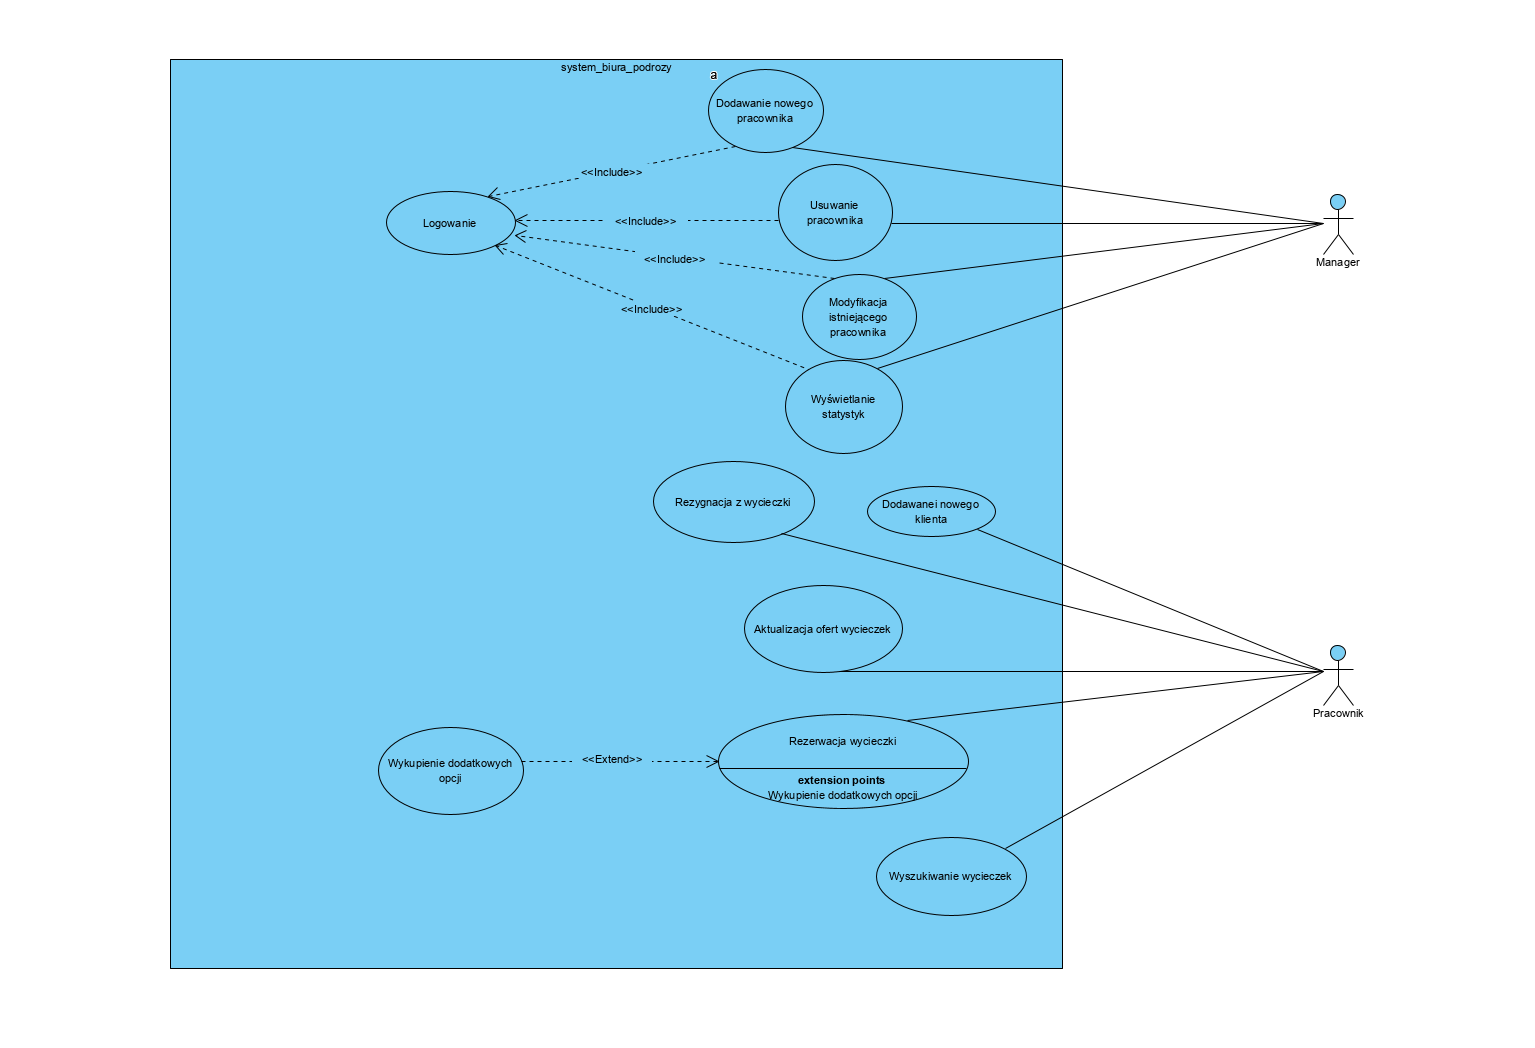
\includegraphics[width=20cm]{use_case.PNG}
Diagram przypadków użycia jest diagramem, który przedstawia funkcjonalność systemu wraz z jego otoczeniem. Diagramy przypadków użycia służą do zobrazowania usług, które są widoczne z zewnątrz systemu. Na diagramie wyróżniamy dwóch aktorów, pracownika oraz managera. Każdemu z nich przyporządkowane są odpowiednie funkcje systemu.

\subsection{Dokumentacja Przypadków Użycia}
\textbf{Nazwa}: Dodawanie nowego pracownika \newline
\textbf{Typ przypadku użycia:} Ogólny, niezbędny \newline
\textbf{Aktorzy:} Manager \newline
\textbf{Krótki opis:} Wprowadzenie danych nowego pracownika do systemu \newline
\textbf{Warunki wstępne:} Manager musi być zalogowany \newline
\textbf{Warunki końcowe:} Nowy pracownik został dodany, może być teraz przypisywany do wycieczek. \newline
\textbf{Główny przepływ zdarzeń:} \newline
1. Manager wypełnia formularz dotyczący nowego pracownika \newline
2. System weryfikuje wprowadzone dane. \newline
3a. Nowy pracownik zostaje dodany \newline
\textbf{Alternatywny przepływ:} \newline
3b. Jeżeli manager podał PESEL nowego pracownika który istnieje już w bazie danych, transakcja
zostaje odrzucona i stosowny komunikat zostaje wyświetlony na ekranie. \newline
3c. Jeżeli manager nie podał wszystkich danych dotyczących pracownika, transakcja zostaje
odrzucona i zostaje wyświetlony stosowny komunikat, następuje powrót do kroku 1. \newline
 \newline
\textbf{Nazwa:} Usuwanie pracownika\newline
\textbf{Typ przypadku użycia:} Ogólny, niezbędny\newline
\textbf{Aktorzy:} Manager\newline
\textbf{Krótki opis:} Usunięcie danych pracownika z systemu, osierocenie wycieczek będących po nadzorem
usuwanego pracownika.\newline
\textbf{Warunki wstępne:} Pracownik którego chcemy usunąć już istnieje w bazie danych. Manager jest
zalogowany.\newline
\textbf{Warunki końcowe:} Pracownik zostaje usunięty z bazy danych, wszystkie wycieczki które nadzorował
zostają osierocone (wartość NULL) – manager powinien wkrótce przypisać tam nowego pracownika.\newline
\textbf{Główny przepływ zdarzeń:}\newline
1.Wybranie pracownika do usunięcia z listy istniejących pracowników.\newline
2.Potwierdzenie usunięcia pracownika przez klikniecie przycisku usuń.\newline
3. Pracownik zostaje usunięty z systemu\newline
4. Wszystkie wycieczki które nadzoruje usuwany pracownik zostają osierocone.\newline
5. Wyświetlenie komunikatu o powodzeniu akcji.\newline
\textbf{Alternatywny przepływ:}\newline
Brak\newline
\newline
\textbf{Nazwa:} Modyfikacja istniejącego pracownika\newline
\textbf{Typ przypadku użycia:} Ogólny, niezbędny\newline
\textbf{Aktorzy:} Manager\newline
\textbf{Krótki opis:} Zmiana (albo aktualizacja) informacji o pracowniku.\newline
\textbf{Warunki wstępne:} Manager jest zalogowany. Pracownik którego chcemy zmodyfikować istnieje w\newline
bazie danych.\newline
\textbf{Warunki końcowe:} Pracownik zostaje usunięty z bazy danych, wszystkie wycieczki które nadzorował\newline
zostają osierocone (wartość NULL) – manager powinien wkrótce przypisać tam nowego pracownika.\newline
\textbf{Główny przepływ zdarzeń:}\newline
1. Wybranie pracownika do modyfikacji z listy istniejących pracowników.\newline
2. Zmiana wybranych danych pracownika w formularzu.\newline
3a. Klikniecie przycisku zapisz zmiany w celu modyfikacji pracownika w bazie danych.\newline
4. Wyświetlenie komunikatu o udanej akcji\newline
\textbf{Alternatywny przepływ:}\newline
3b. Wypełnione pola w formularza posiadają niepoprawne dane. Następuje przejście do kroku 2.\newline
\newline
\textbf{Nazwa:} Wyświetlanie statystyk\newline
Typ przypadku użycia: Ogólny, niezbędny\newline
\textbf{Aktorzy:} Manager\newline
\textbf{Krótki opis:} Wyświetlanie statystyk z informacjami na temat dochodów firmy.\newline
\textbf{Warunki wstępne:} Manager jest zalogowany\newline
\textbf{Warunki końcowe:} Wyświetlone zostają przeanalizowane statystyki.\newline
\textbf{Główny przepływ zdarzeń:}\newline
1. Kliknięcie na przycisk wygeneruj statystyki\newline
2. Wyświetlenie statystyk\newline
\textbf{Alternatywny przepływ:}\newline
Brak\newline
\newline
\textbf{Nazwa:} Logowanie\newline
\textbf{Aktorzy:} Manager\newline
\textbf{Krótki opis:} Logowanie do systemu\newline
\textbf{Warunki wstępne:} Osoba logująca posiada konto managera.\newline
\textbf{Warunki końcowe:} Autentykacja przechodzi poprawnie.\newline
\textbf{Główny przepływ zdarzeń:}\newline
1. Wpisanie nazwy użytkownika oraz hasła do formularza logowania\newline
2. Zatwierdzenie formularza\newline
3. Weryfikacja danych\newline
4a. Przyznanie dostępu do panelu managera\newline
\textbf{Alternatywny przepływ zdarzeń:}\newline
4b. W przypadku niepowodzenia wyświetlony zostaje komunikat o niepowodzeniu operacji.\newline
Następuje powrót do kroku 1.\newline
\newline
\textbf{Nazwa:} Wyszukiwanie wycieczek\newline
\textbf{Aktorzy:} Pracownik\newline
\textbf{Krótki opis:} Pracownik wyszukuje wycieczek na podstawie kryteriów dostarczonych przez klienta oraz\newline
własnych propozycji.\newline
\textbf{Warunki wstępne:} Brak\newline
\textbf{Warunki końcowe:} Otrzymanie listy wycieczek zgodnych z wprowadzonymi kryteriami.\newline
\textbf{Główny przepływ zdarzeń:}\newline
1. Pracownik wprowadza kryteria wyszukiwania do formularza.\newline
2a. Pracownik otrzymuje listę wycieczek spełniających przestawione kryteria.\newline
\textbf{Alternatywny przepływ zdarzeń:}\newline
2b. Jeżeli wynik nie jest satysfakcjonujący, następuje powrót do kroku 1.\newline
\newline
\textbf{Nazwa:} Aktualizacja ofert wycieczek\newline
\textbf{Aktorzy:} Pracownik\newline
\textbf{Krótki opis:} Dodanie informacji o nowej wycieczce do oferty biura podróży.\newline
\textbf{Warunki wstępne:} Wycieczka nie figuruje w systemie.\newline
\textbf{Warunki końcowe:} Wycieczka zostaje dodana do oferty biura podróży.\newline
\textbf{Główny przepływ zdarzeń:}\newline
1. Wypełnienie pól dotyczących nowej wycieczki\newline
2. Kliknięcie przycisku dodaj wycieczkę\newline
3a. Zostaje wyświetlony komunikat o poprawnie dodanej wycieczce\newline
\textbf{Alternatywny przepływ:}\newline
3b. Zostaje wyświetlony komunikat o błędnie wprowadzonych danych następuje powrót do\newline
kroku 1.\newline
\newline
\textbf{Nazwa:} Rezygnacja z wycieczki\newline
\textbf{Aktorzy:} Pracownik\newline
\textbf{Krótki opis:} Usunięcie wycieczki zarezerwowanej/wykupionej przez klienta.\newline
\textbf{Warunki wstępne:} Klient posiada wykupioną wycieczkę.\newline
\textbf{Warunki końcowe:} Wycieczka zostaje usunięta.\newline
\textbf{Główny przepływ zdarzeń:}\newline
1. Wypełnienie formularza danymi pozwalającymi wyszukać wykupioną wycieczkę.\newline
2. Wybranie wycieczki spośród znalezionych ofert.\newline
3. Usunięcie zarezerwowanej wycieczki za pomocą przycisku usuń wycieczkę.\newline
\newline
\textbf{Nazwa:} Rezerwacja wycieczki\newline
\textbf{Typ przypadku użycia:} Ogólny, niezbędny\newline
\textbf{Aktorzy:} Pracownik\newline
\textbf{Krótki opis:} Dodanie nowej rezerwacji do tabeli z zarezerwowanymi/wykupionymi wycieczkami.\newline
\textbf{Warunki wstępne:} Klient oraz rezerwowana wycieczka istnieje w bazie danych. Ilość dostępnych\newline
miejsc dotyczących danej wycieczki nie została wyczerpana.\newline
\textbf{Warunki końcowe:} Nowa rezerwacja zostaje dodana do systemu.\newline
\textbf{Główny przepływ zdarzeń:}\newline
1. Wypełnienie pól dotyczących wyszukiwanej wycieczki\newline
2a. Wybranie znalezionej wycieczki\newline
3. Wypełnienie pól dotyczących danego klienta\newline
4a. Wybranie znalezionego klienta\newline
5a. Wybranie dodatkowych opcji\newline
6. Kliknięcie na przycisk dokonaj rezerwacji\newline
\textbf{Alternatywny przepływ:}\newline
2b. W przypadku braku znalezionych wycieczek, zostaje wyświetlony stosowny komunikat.\newline
Następuje powrót do kroku 1.\newline
4b. W przypadku braku znalezionych klientów, zostaje wyświetlony stosowny komunikat.\newline
Następuje powrót do kroku 3.\newline
5b Pominięcie dodatkowych opcji
\section{Projekt, implementacja i testy bazy danych}
\subsection{Wymagania dostępu do bazy}
Każdy użytkownik w zależności od typu konta może wykonywać różne operacja na tabelach. Poniżej tabela z uprawnieniami dla poszczególnych operacji(CRUD) na encjach bazy danych.

\begin{center}
 \begin{tabular}{|c c c c c|} 
  \hline
 \multicolumn{5}{|c|}{Uprawnienia Manager(hiprio)} \\
 \hline
 Nazwa tabeli  & Create & Read & Update & Delete\\ [0.3ex] 
 \hline\hline
 Tour & + & +  & + & +\\ 
 \hline
 Customers  & +  & +  & +  & +  \\
 \hline
 Offers  & + & +  & +  & +\\
 \hline
 Extras  & +  & +  & +  & + \\
 \hline
 Category  & +  & +  & +  & + \\ [1ex] 
 \hline
 Employees  & +  & +  & +  & + \\ [1ex] 
 \hline
 Credentials  & +  & +  & +  & + \\ [1ex] 
 \hline
\end{tabular}
\end{center}

\begin{center}
 \begin{tabular}{|c c c c c|} 
  \hline
 \multicolumn{5}{|c|}{Uprawnienia Pracownik(miprio)} \\
 \hline
 Nazwa tabeli  & Create & Read & Update & Delete\\ [0.3ex] 
 \hline\hline
 Tour & + & +  & + & +\\ 
 \hline
 Customers  & +  & +  & +  & +  \\
 \hline
 Offers  & + & +  & +  & +\\
 \hline
 Extras  & +  & +  & +  & + \\
 \hline
 Category  & +  & +  & +  & + \\ [1ex] 
 \hline
 Employees  & -  & -  & -  & - \\ [1ex] 
 \hline
 Credentials  & -  & -  & -  & - \\ [1ex] 
 \hline
\end{tabular}
\end{center}

\begin{center}
 \begin{tabular}{|c c c c c|} 
  \hline
 \multicolumn{5}{|c|}{Uprawnienia początkowe(loprio)} \\
 \hline
 Nazwa tabeli  & Create & Read & Update & Delete\\ [0.3ex] 
 \hline\hline
 Tour & - & -  & - & -\\ 
 \hline
 Customers  & -  & -  & -  & -  \\
 \hline
 Offers  & - & -  & -  & -\\
 \hline
 Extras  & -  & -  & -  & - \\
 \hline
 Category  & -  & -  & -  & - \\ [1ex] 
 \hline
 Employees  & -  & -  & -  & - \\ [1ex] 
 \hline
 Credentials  & -  & +  & -  & - \\ [1ex] 
 \hline
\end{tabular}
\end{center}
Komendy użyte do stworzenia oraz nadania uprawnień użytkoniwkom.
\begin{lstlisting}
create user 'loprio'@'localhost' identified by 'bazydanych19';
grant usage on *.* to 'loprio'@'localhost';
revoke select, alter, create, delete, drop, insert, index, references, update  on table *.* from 'loprio'@'localhost';
grant select, show view  on table `biuro_podrozy`.`credentials`
to 'loprio'@'localhost';
grant select, show view  on table `biuro_podrozy`.`employees`
to 'loprio'@'localhost';
grant select, show view  on table `biuro_podrozy_test`.`credentials`
to 'loprio'@'localhost';
grant select, show view  on table `biuro_podrozy_test`.`employees`
to 'loprio'@'localhost';
flush privileges;

create user 'miprio'@'localhost' identified by 'bazydanych19';
grant usage on *.*
to 'miprio'@'localhost';
revoke select, alter, create, delete, drop, insert, index, references, update  on table *.* from 'miprio'@'localhost';
grant all privileges  on table `biuro_podrozy`.`annual_income`
to 'miprio'@'localhost';
grant all privileges  on table  `biuro_podrozy`.`category`
to 'miprio'@'localhost';
grant all privileges  on table  `biuro_podrozy`.`customers`
to 'miprio'@'localhost';
grant all privileges  on table  `biuro_podrozy`.`offers`
to 'miprio'@'localhost';
grant all privileges  on table  `biuro_podrozy`.`tour`
to 'miprio'@'localhost';
grant all privileges  on table `biuro_podrozy_test`.`annual_income`
to 'miprio'@'localhost';
grant all privileges  on table  `biuro_podrozy_test`.`category`
to 'miprio'@'localhost';
grant all privileges  on table  `biuro_podrozy_test`.`customers`
to 'miprio'@'localhost';
grant all privileges  on table  `biuro_podrozy_test`.`offers`
to 'miprio'@'localhost';
grant all privileges  on table  `biuro_podrozy_test`.`tour`
to 'miprio'@'localhost';
flush privileges;

create user 'hiprio'@'localhost' identified by 'bazydanych19';
grant usage on *.*
to 'hiprio'@'localhost';
grant all privileges  on table `biuro_podrozy`.*
to 'hiprio'@'localhost';
grant all privileges  on table `biuro_podrozy_test`.*
to 'hiprio'@'localhost';
flush privileges;

create user 'superuser'@'localhost' identified by '';
grant usage on *.*
to 'superuser`'@'localhost';
grant all privileges  on table *.*
to 'superuser`'@'localhost';
flush privileges;


\end{lstlisting}
\subsection{Diagram ERD}
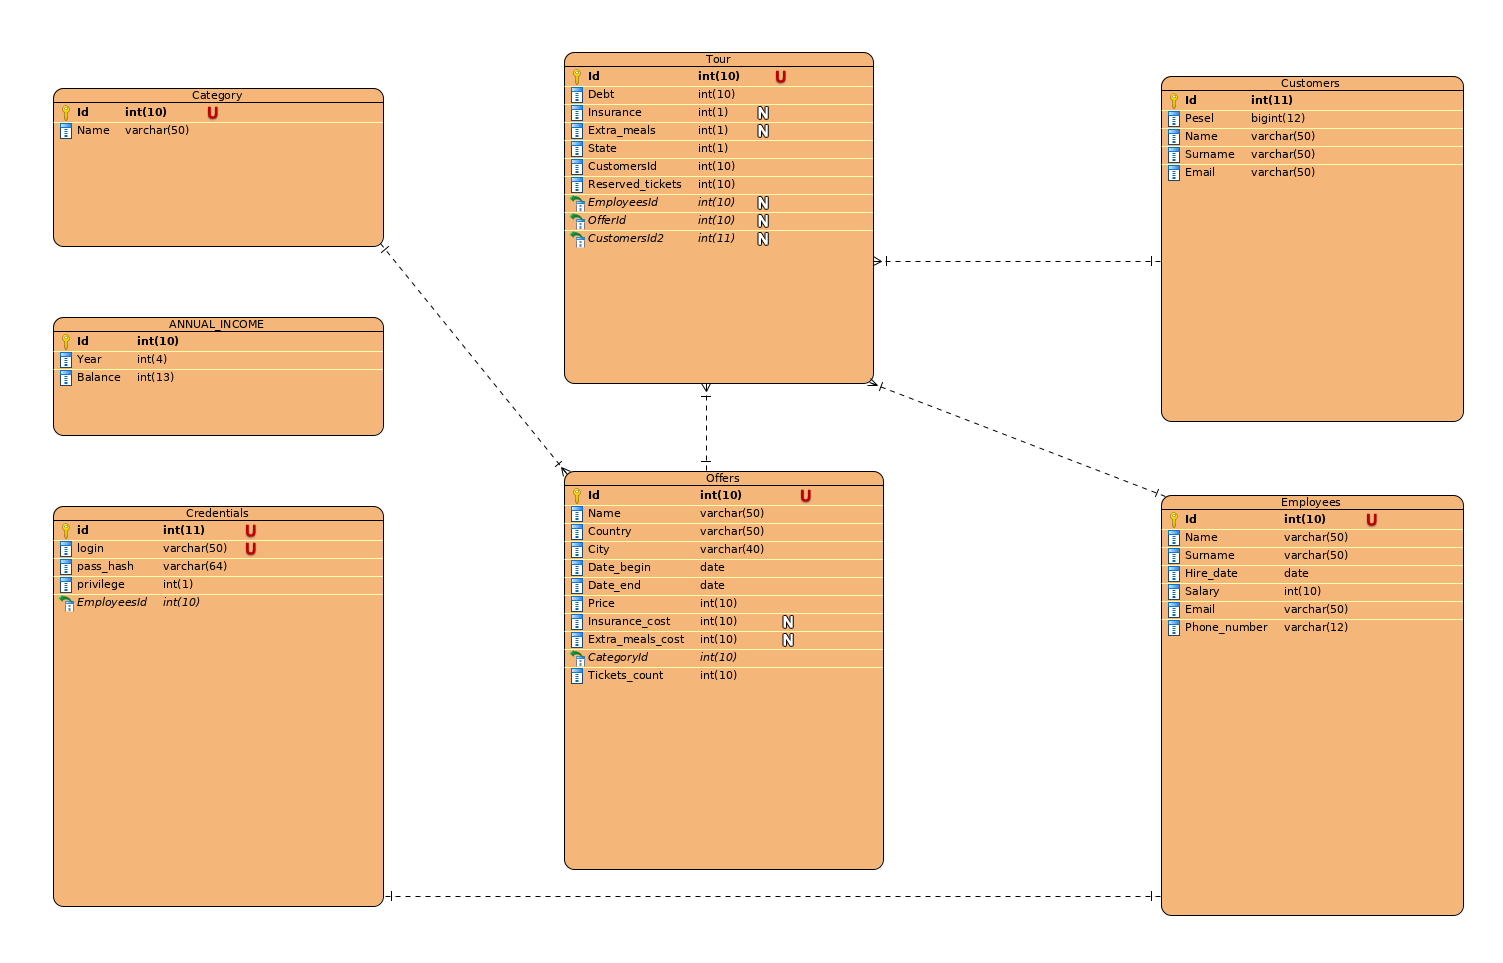
\includegraphics[width=18cm]{ERD_diagram.png}
\subsection{Normalizacja modelu bazy danych}
Postać normalna to postać relacji w bazie danych, która nie zawiera nadmiarowych(powtarzając się) danych. Proces normalizacji polega na przeprowadzeniu analizy bazy danych pod kątem redundantnych rekordów oraz wyeliminowania ich. Zaprojektowana przez z nas baza danych nie wymagała normalizacji. 
\subsection{Opis fizycznego modelu bazy danych}
Silnikiem bazodanowym który wybraliśmy jest MariaDB. Serwer ten jest całkowicie darmowy, oraz należy do grupy aplikacji  z otwartym kodem źródłowym.
MariaDB jest sql'owym systemem relacyjnym, posiadającym otwarte API w różnych językach programowania.
Do komunikacji z bazą danych zastosowany został język SQL. Poniżej wybrane procedury realizujące implementacje modelu bazy danych oraz umożliwiające jej modyfikacje.
\begin{lstlisting}
-- tworzenie bazy danych
create database biuro_podrozy character set UTF8MB4;

-- tworzenie tabeli z rezerwacjami 
CREATE TABLE BIURO_PODROZY.Tour (
  Id               int(10) NOT NULL AUTO_INCREMENT, 
  Debt             int(10) NOT NULL, 
  Insurance        int(1),
  Extra_meals      int(1), 
  Finished         int(1) NOT NULL, 
  Reserved_tickets int(10) NOT NULL, 
  CustomerPesel    bigint(12), 
  EmployeeId       int(10), 
  OfferId          int(10), 
  PRIMARY KEY (Id));

 -- Dodanie kluczy obcych do tabeli z wycieczkami 
 ALTER TABLE BIURO_PODROZY.Tour ADD CONSTRAINT FKTour997364 FOREIGN KEY (CustomerPesel) REFERENCES BIURO_PODROZY.Customers (Pesel);

 -- Dodanie nowej rezerwacji
 INSERT INTO BIURO_PODROZY.TOUR 
  (OFFERID, CustomerPesel, EMPLOYEEID, Insurance, Extra_meals, DEBT, FINISHED, RESERVED_TICKETS) 
VALUES 
  (28,92121963645,41,1,0,1379,1,2);
 
-- trigger modyfikujacy pole w tabeli tour w momencie usunięcia pracownika.
-- W każdej rezerwacji z przypisanym niejstniejącym pracownikiem modyfikowane jest
-- pole z id pracownika tak, aby nie wskazywało na niestniejącego pracownika.  
CREATE TRIGGER on_employee_remove
AFTER DELETE ON BIURO_PODROZY.Employees 
FOR EACH ROW 
UPDATE BIURO_PODROZY.Tour
SET Tour.EmployeeId = NULL WHERE Tour.EmployeeId = OLD.Id;

-- procedura rezerwacji wycieczki
delimiter //

CREATE PROCEDURE reserve_tour (
  IN offerid INT,
  IN ticket_count INT,
  IN customerid BIGINT,
  IN employeeid INT,
  IN Insurance INT(1),
  IN extra_meals INT(1)
)
proc_begin:BEGIN
  DECLARE offer_ticket_count INT DEFAULT 0;
  DECLARE offer_Insurance_cost INT;
  DECLARE offer_extra_meals_cost INT;
  DECLARE offer_price INT;
  
  SELECT Tickets_count, price, Insurance_cost, Extra_meals_cost
  INTO offer_ticket_count, offer_price, offer_Insurance_cost, offer_extra_meals_cost
  FROM Offers WHERE Offers.Id = offerid;
  
  IF offer_ticket_count < ticket_count THEN
    LEAVE proc_begin;
  END IF;
  
  SET offer_price = offer_price*ticket_count;
  
  IF offer_Insurance_cost IS NOT NULL AND Insurance <> 0 THEN
    SET offer_price = offer_price + offer_Insurance_cost*ticket_count;
  END IF;
  
  IF offer_extra_meals_cost IS NOT NULL AND extra_meals <> 0 THEN
    SET offer_price = offer_price + offer_extra_meals_cost*ticket_count;
  END IF;
  
  INSERT INTO BIURO_PODROZY.TOUR 
  (OfferId, CustomerPesel, EMPLOYEEID, Insurance, Extra_meals, DEBT, FINISHED, RESERVED_TICKETS) 
VALUES 
  (offerid,customerid,employeeid,Insurance,extra_meals,offer_price,0,ticket_count);
END//
\end{lstlisting}

Zdefiniowane zostały również wyzwalacze, które automatyzują operacje na bazie danych po wykonaniu akcji na tabelach oraz procedury które przyspieszają wykonanie złożonych operacji na bazie danych wymagających wykorzystania kilku tabel.\newline
Poniżej kilka przykładów wyzwalaczy oraz procedur z krótkim komentarzem w kodzie.\newline
\begin{lstlisting}
-- zdefinowanie wyzwalacza uruchomianego po dodaniu nowej tury
-- wyzwalacz odejmuje zdefinowana liczbe zarezerwowanych biletow
-- od liczby dostepnych bieltow dla danej oferty
create trigger on_new_tour_appear
after insert on biuro_podrozy.tour
for each row
update biuro_podrozy.offers
  set offers.tickets_count = offers.tickets_count - new.reserved_tickets
  where offers.id = new.offerid;


-- zdefinowanie wyzwalacza uruchomianego po usunieciu pracownika
-- wyzwalacz usuwa przypisanie pracownika z wszystkich
-- przypisanych do niego wycieczek
create trigger on_employee_remove
after delete on biuro_podrozy.employees
for each row
update biuro_podrozy.tour
  set tour.employeeid = null where tour.employeeid = old.id;


-- procedura rezerwujaca nowa wycieczke
-- na bazie otrzymanych kluczy obcych, pobierane sa wymagane dane,
-- nastepnie obliczany jest calkowity koszt wycieczki i dodanie jej
create procedure reserve_tour (
  in offerid int,
  in ticket_count int,
  in customerid bigint,
  in employeeid int,
  in insurance int(1),
  in extra_meals int(1)
)
proc_begin:begin
  declare offer_ticket_count int default 0;
  declare offer_insurance_cost int;
  declare offer_extra_meals_cost int;
  declare offer_price int;

  select tickets_count, price, insurance_cost, extra_meals_cost
  into offer_ticket_count, offer_price, offer_insurance_cost, offer_extra_meals_cost
  from offers where offers.id = offerid;

  if offer_ticket_count < ticket_count then
    leave proc_begin;
  end if;

  set offer_price = offer_price*ticket_count;

  if offer_insurance_cost is not null and insurance <> 0 then
    set offer_price = offer_price + offer_insurance_cost*ticket_count;
  end if;

  if offer_extra_meals_cost is not null and extra_meals <> 0 then
    set offer_price = offer_price + offer_extra_meals_cost*ticket_count;
  end if;

  insert into biuro_podrozy.tour
  (offerid, customerid, employeeid, insurance, extra_meals, debt, state, reserved_tickets)
values
  (offerid,customerid,employeeid,insurance,extra_meals,offer_price,0,ticket_count);


-- procedura wylicajaca koszt zarezerwowanej wycieczki
-- po rezygnacji z ubezpieczenia
create procedure resign_from_insurance (
  in tourid int
)
proc_begin:begin
  declare withinsurance int(1);
  declare tour_state int(1);
  declare tour_debt int;
  declare tour_reserved_tickets int;
  declare tour_offerid int;
  declare offer_insurance_cost int;

  select insurance, debt, reserved_tickets, state, offerid
  into withinsurance, tour_debt, tour_reserved_tickets, tour_state, tour_offerid
  from tour where  tour.id = tourid;

  if withinsurance is null or withinsurance = 0 or tour_state = 1 then
    leave proc_begin;
  end if;

  select insurance_cost
  into offer_insurance_cost
  from offers where  offers.id = tour_offerid;

  set tour_debt = tour_debt -  offer_insurance_cost*tour_reserved_tickets;

  update biuro_podrozy.tour
     set
        tour.debt = tour_debt,
        tour.insurance =0
     where tour.id = tourid;
end//
\end{lstlisting}
\section{Projekt, implementacja i testy aplikacji bazodanowej}
\subsection{Makieta interfejsu bazodanowej aplikacji}

\bibliographystyle{abbrv}
\bibliography{ref}
\end{document}

